\documentclass[12pt]{article}

\usepackage[T2A]{fontenc}
\usepackage[utf8]{inputenc}
\usepackage[russian]{babel}

\usepackage{amsmath,amssymb,mathtools}
\usepackage{geometry}
\usepackage{float}
\usepackage{placeins}
\usepackage{hyperref}

\geometry{margin=2.5cm}

\setlength{\parindent}{0pt}
\setlength{\parskip}{4pt}

\newcommand{\dd}{\mathrm{d}}
\newcommand{\pd}[2]{\frac{\partial #1}{\partial #2}}
\newcommand{\pdd}[2]{\frac{\partial^2 #1}{\partial #2^2}}

\title{Краткий обзор end-to-end стратегии}
\author{Ширяев Е.\ А.}
\date{}

\begin{document}

\maketitle

\noindent Юпитер ноутбук: \href{https://github.com/tenzenmonsta/End-to-end-quant-strategy}{End to end GH}

\section{Формулировка торговой гипотезы и её мотивация}
\textbf{Гипотеза:} на рынке ликвидных российских акций наблюдаются устойчивые среднесрочные тренды.
Комбинация \textit{trend-following} и \textit{volatility targeting} улучшает риск-профиль портфеля относительно пассивного владения.

\medskip
\textbf{Ожидаемый эффект:}
\begin{itemize}
    \item участие в направленных движениях рынка;
    \item снижение риска в периоды высокой волатильности;
\end{itemize}

\subsection*{Экономическая мотивация}
\begin{itemize}
    \item \textbf{Momentum:} активы с положительной динамикой часто продолжают движение.
    \item \textbf{Кластеризация волатильности:} управление позицией через \textit{target vol} стабилизирует риск.
\end{itemize}

\subsection*{Идея реализации}
Стратегия использует тренд-фильтр и масштабирование позиций по целевой волатильности для получения более стабильной риск-скорректированной доходности относительно пассивного равновзвешенного портфеля.


\subsection*{Критерии принятия стратегии в прод}

\begin{enumerate}
    \item \textbf{Out-of-sample устойчивость}
    \begin{itemize}
        \item стабильные результаты на walk-forward периодах;
        \item контролируемый уровень просадок.
    \end{itemize}

    \item \textbf{Устойчивость к издержкам}
    \begin{itemize}
        \item стратегия остаётся жизнеспособной при реалистичных комиссиях и спрэдах;
    \end{itemize}

    \item \textbf{Робастность параметров}
    \begin{itemize}
        \item небольшие изменения \textit{lookback} / \textit{vol-target} не должны ломать стратегию;
    \end{itemize}

    \item \textbf{Контроль риска}
    \begin{itemize}
        \item ограниченный \textit{max drawdown};
        \item стабильная волатильность портфеля;
    \end{itemize}

    \item \textbf{Реализуемость}
    \begin{itemize}
        \item используются ликвидные инструменты;
        \item разумная частота ребалансировки.
    \end{itemize}
\end{enumerate}
\section{Получение и выгрузка данных}

Данные загружались через API Т-Банка (\textit{Tinkoff Invest API}): исторические свечи по инструментам и дивиденды.

В проекте использовались синхронный и асинхронный режимы загрузки. Асинхронная часть загрузки ускоряет сбор данных по нескольким инструментам: пока один запрос ожидает ответ от API, программа может выполнять другие запросы.

\section{Обработка ценовых данных}

После получения данных от брокера ценовые ряды необходимо привести к единому и пригодному для бэктеста виду. В рамках проекта обработка включала два основных этапа:
\begin{itemize}
    \item обработку пропусков в ценовых рядах;
    \item корректировку цен на дивиденды.
\end{itemize}

\subsection*{Обработка пропусков}

Для обработки пропусков использовалась схема \texttt{ffill().dropna()}:
\begin{itemize}
    \item \texttt{ffill()} --- заполнение пропусков последним доступным значением цены;
\end{itemize}

Выбор \texttt{ffill()} обусловлен тем, что он использует только информацию, доступную на момент наблюдения, и не приводит к утечке данных из будущего. Это важно для корректного бэктеста и расчёта торговых сигналов.

Подход \texttt{bfill()} (заполнение значением из будущего) не использовался, поскольку он может вносить \textit{look-ahead bias}. По той же причине не применялась схема \texttt{ffill().bfill()}: несмотря на формальное устранение большего числа пропусков, такой подход может заполнять значения будущими ценами и делать результаты бэктеста методологически некорректными.

\subsection*{Корректировка цен на дивиденды}

Для корректного расчёта ценовых доходностей использовалась аддитивная корректировка цен на дивиденды. Без такой корректировки на дивидендных отсечках в ценовом ряду возникают скачки вниз, которые не связаны с рыночным движением и могут искажать доходности, волатильность и торговые сигналы.

\subsubsection*{Идея корректировки}
Пусть $P_t$ --- цена в момент $t$, $D_u$ --- дивидендная выплата на акцию в момент $u$, а $P_t^{adj}$ --- скорректированная цена. Тогда аддитивная корректировка задаётся как
\[
P_t^{adj} = P_t - \sum_{u>t} D_u.
\]

Иными словами, из исторической цены вычитается сумма будущих дивидендов, чтобы убрать эффект дивидендных отсечек из ценового ряда.

\subsubsection*{Особенности реализации}
В реализации использовались данные о дивидендах по инструментам с последующим накоплением будущих выплат по временной шкале. Дополнительно учитывались сплиты: для дивидендов до даты сплита значения пересчитывались с учётом коэффициента сплита, чтобы корректировка оставалась сопоставимой с текущим масштабом цен.

\subsubsection*{Комментарий по валидации}
При желании корректировки можно сверять с внешними источниками (например, \textit{yfinance}), однако абсолютные значения скорректированных цен могут отличаться из-за различий в методике учёта дивидендов и корпоративных событий. Поэтому при сравнении корректнее сопоставлять не уровни цен, а производные величины, в первую очередь доходности (\texttt{pct\_change()}).

\section{Формирование benchmark: равновзвешенный портфель}

В качестве benchmark использовался пассивный равновзвешенный портфель из выбранных ликвидных акций. Такой benchmark позволяет сравнивать результаты стратегии не с отдельным инструментом, а с базовой диверсифицированной альтернативой ``купил и держи'' на том же наборе бумаг.

\subsection*{Принцип построения}
На каждой дате ребалансировки капитал распределяется между всеми активами равными долями. Если в портфель входит $N$ инструментов, то вес каждого инструмента задаётся как
\[
w_i = \frac{1}{N}, \qquad i = 1, \dots, N.
\]
\begin{figure}[h!]
    \centering
    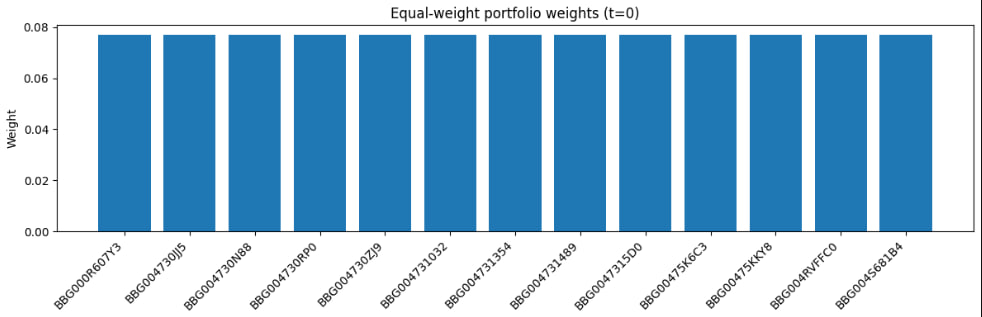
\includegraphics[width=\linewidth]{equal_portfolio}
    \caption{Начальные веса равновзвешенного benchmark-портфеля.}
    \label{fig:benchmark_weights}
\end{figure}

\subsection*{Первичный анализ benchmark-портфеля}

После построения benchmark-портфеля был выполнен базовый диагностический анализ его свойств, чтобы получить ориентир для дальнейшего сравнения со стратегией.

\textbf{Распределение дневных доходностей.}
Гистограмма дневных доходностей benchmark-портфеля позволяет оценить форму распределения, наличие асимметрии и характер хвостов.

\begin{figure}[H]
    \centering
    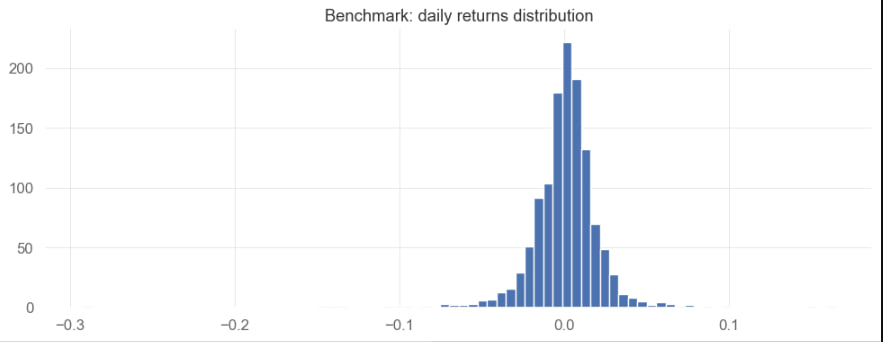
\includegraphics[width=0.82\linewidth]{benchmark_returns_distribution}
    \caption{Распределение дневных доходностей benchmark-портфеля.}
    \label{fig:benchmark_returns_distribution}
\end{figure}

\textbf{QQ-plot дневных доходностей.}
QQ-plot используется для визуальной проверки отклонений распределения доходностей от нормального.

\begin{figure}[H]
    \centering
    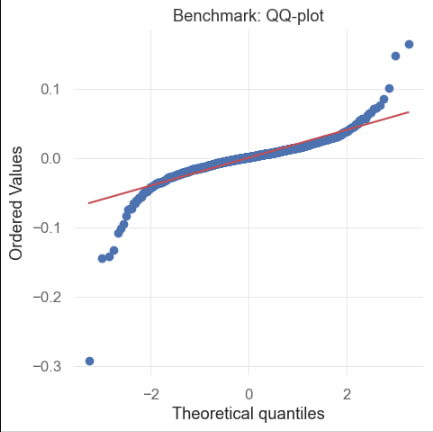
\includegraphics[width=0.55\linewidth]{benchmark_qqplot}
    \caption{QQ-plot дневных доходностей benchmark-портфеля.}
    \label{fig:benchmark_qqplot}
\end{figure}

По результатам первичной диагностики benchmark-портфеля можно оценить форму распределения доходностей и возможные отклонения от нормальности.

\FloatBarrier
\clearpage

\textbf{Корреляционная структура активов.}
Корреляционная матрица показывает степень совместного движения бумаг и позволяет оценить фактическую диверсификацию benchmark-портфеля.

\begin{figure}[H]
    \centering
    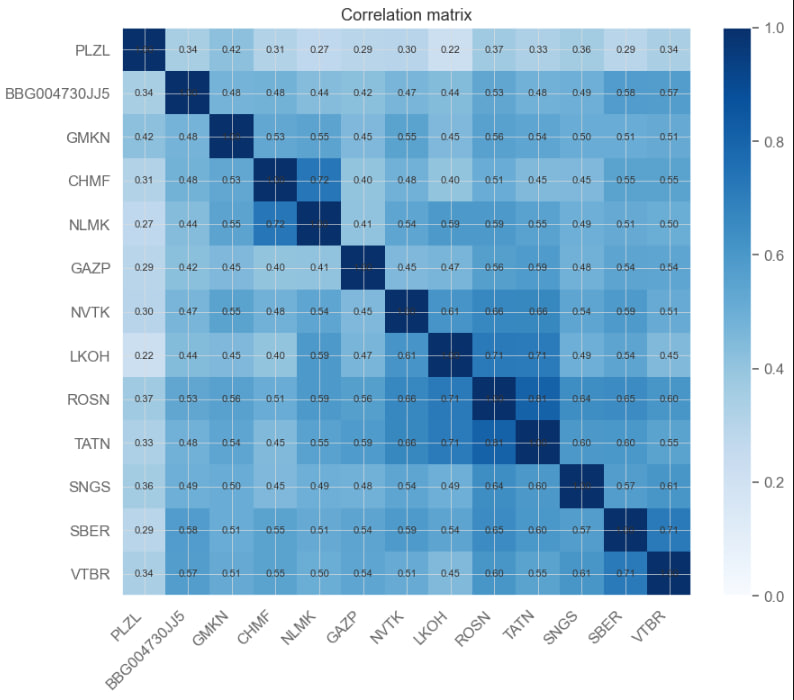
\includegraphics[width=0.88\linewidth]{benchmark_corr_matrix}
    \caption{Корреляционная матрица доходностей активов benchmark-портфеля.}
    \label{fig:benchmark_corr_matrix}
\end{figure}


\FloatBarrier

\section{Торговая стратегия: тренд-фильтр и volatility targeting}

Стратегия строится как надстройка над benchmark-портфелем (равновзвешенным портфелем акций). Вместо выбора отдельных бумаг стратегия управляет экспозицией к benchmark: увеличивает или снижает долю капитала в базовом портфеле в зависимости от рыночного режима и текущей волатильности.

\subsection*{Основная идея}
Используются два простых и интерпретируемых правила:
\begin{itemize}
    \item \textbf{тренд-фильтр:} риск держится только тогда, когда кривая капитала benchmark выше своей скользящей средней;
    \item \textbf{volatility targeting:} размер позиции масштабируется так, чтобы поддерживать целевой уровень волатильности стратегии.
\end{itemize}

Таким образом, стратегия сочетает фильтрацию неблагоприятных рыночных режимов с контролем риска через динамическое управление экспозицией.

\subsection*{Формализация}
Пусть \(r_t^{(b)}\) --- доходность benchmark-портфеля, а \(x_t\) --- экспозиция стратегии к benchmark.

\textbf{1) Тренд-фильтр.}  
По доходностям benchmark строится equity curve:
\[
E_t = \prod_{u \le t}(1+r_u^{(b)}).
\]
Если \(E_t\) выше своей скользящей средней, риск ``включён'', иначе экспозиция снижается.

\textbf{2) Volatility targeting.}  
Оценка реализованной волатильности \(\widehat{\sigma}_t\) рассчитывается по скользящему окну. Целевая экспозиция задаётся как
\[
x_t \propto \frac{\sigma^\star}{\widehat{\sigma}_t},
\]
где \(\sigma^\star\) --- целевая годовая волатильность. На практике экспозиция ограничивается сверху (ограничение на плечо).

\textbf{3) Доходность стратегии.}  
Для корректного бэктеста используется лагированная экспозиция \(x_{t-1}\) (без look-ahead bias). Тогда доходность стратегии складывается из доходности benchmark и доходности кэша:
\[
r_t^{(\text{strat})} = x_{t-1} r_t^{(b)} + (1-x_{t-1}) r_t^{(cash)} - c_t,
\]
где \(c_t\) --- издержки ребалансировки, пропорциональные изменению экспозиции.

\subsection*{Диагностика доходностей стратегии}

Для первичной диагностики результатов стратегии анализируется распределение дневных доходностей. Гистограмма позволяет визуально оценить концентрацию наблюдений около нуля, асимметрию и наличие хвостов распределения.

\begin{figure}[H]
    \centering
    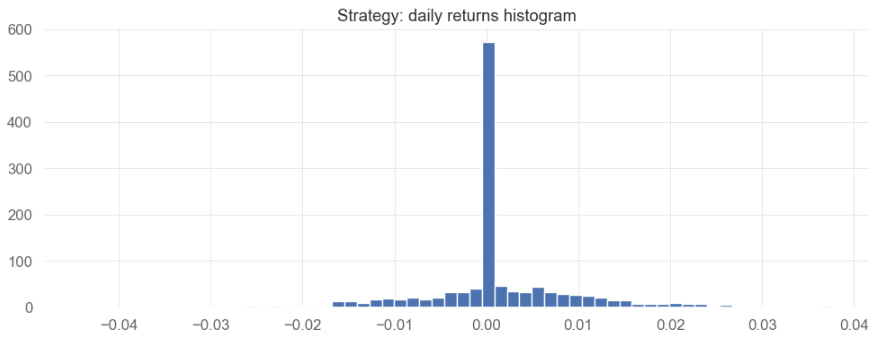
\includegraphics[width=0.82\linewidth]{strategy_returns_hist}
    \caption{Гистограмма дневных доходностей стратегии.}
    \label{fig:strategy_returns_hist}
\end{figure}

Высокая концентрация значений вблизи нуля связана с периодами пониженной или нулевой экспозиции к benchmark-портфелю (например, при выключенном тренд-фильтре), а также с влиянием сглаживания экспозиции и кэш-компоненты. 
\subsection*{6. Walk-forward валидация с embargo}

Для оценки устойчивости результатов использовалась walk-forward out-of-sample валидация по временным рядам с embargo-разрывом между обучающим и тестовым окнами.

На каждом шаге формировалось историческое окно (\(L_{\text{back}}\)), затем задавался embargo-разрыв (\(L_{\text{emb}}\)), после чего качество оценивалось на последующем тестовом интервале (\(L_{\text{fwd}}\)). Далее окно сдвигалось вперёд, и процедура повторялась.

Embargo вводится для того, чтобы уменьшить утечку информации между соседними окнами и снизить лишнюю корреляцию между out-of-sample метриками на соседних шагах валидации.

\begin{figure}[H]
    \centering
    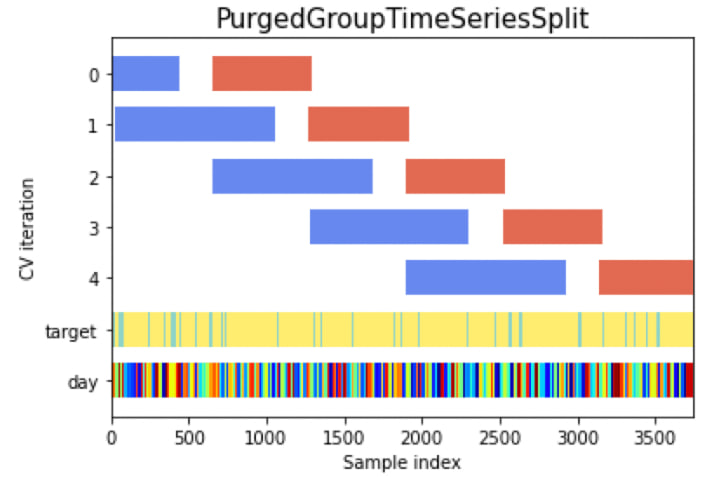
\includegraphics[width=0.62\linewidth]{walkforward_embargo_scheme}
    \caption{Схема walk-forward валидации с embargo-разрывом.}
    \label{fig:walkforward_embargo_scheme}
\end{figure}

\subsection*{Получение out-of-sample метрик}

После выполнения walk-forward валидации для каждого out-of-sample окна рассчитывались ключевые метрики качества: \textit{Total Return}, \textit{Annualized Return}, \textit{Annualized Volatility}, \textit{CVaR}, \textit{Sharpe Ratio} и \textit{Drawdown}. Это позволяет анализировать не только средний результат, но и разброс метрик по различным рыночным режимам.

Для итоговой диагностики строилось распределение полученных метрик по всем OOS-окнам, что даёт более устойчивое представление о поведении benchmark-портфеля во времени.

\begin{figure}[H]
    \centering
    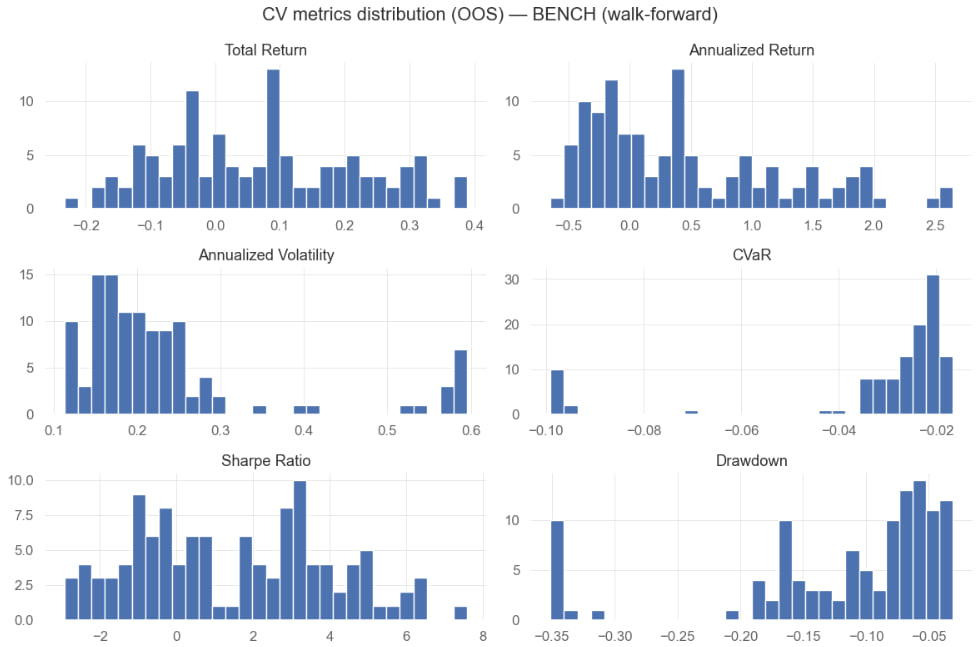
\includegraphics[width=0.92\linewidth]{metrics}
    \caption{Распределение out-of-sample метрик}
    \label{fig:oos_metrics_distribution_bench}
\end{figure}

\subsection*{7. Результаты бэктеста: PnL, equity и сравнение с benchmark}

После задания правил стратегии (тренд-фильтр, volatility targeting, кэш-компонента и издержки) выполнялся бэктест на историческом ряде доходностей benchmark-портфеля. По результатам бэктеста рассчитывались дневные доходности стратегии \(r_t^{(\text{strat})}\), на основе которых строились кривая капитала (\textit{equity}) и накопленный PnL.

Для интерпретации результатов использовались следующие представления:
\begin{itemize}
    \item накопленный PnL стратегии;
    \item накопленный PnL benchmark-портфеля (\textit{buy-and-hold}) для сравнения;
    \item накопленные издержки ребалансировки;
    \item кривая капитала стратегии (\textit{Market Value});
    \item внутримесячный PnL с обнулением в начале каждого месяца (\textit{monthly-reset PnL}).
\end{itemize}

График \textit{monthly-reset PnL} используется как более читаемое представление локальной динамики стратегии: он позволяет визуально оценивать внутримесячные движения, просадки и восстановление без накопления эффекта длинного горизонта.

\begin{figure}[H]
    \centering
    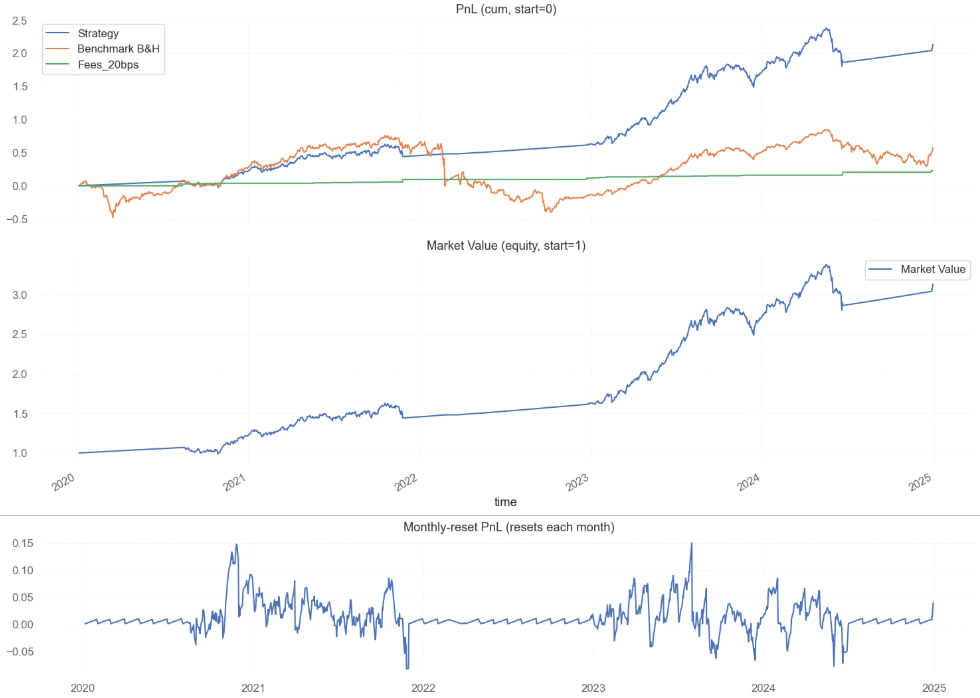
\includegraphics[width=0.95\linewidth]{results}
    \caption{Результаты бэктеста стратегии: накопленный PnL, кривая капитала и monthly-reset PnL.}
    \label{fig:backtest_results}
\end{figure}

\subsection*{8. Итоговые результаты, сравнение метрик и выводы}

На завершающем этапе были рассчитаны и сопоставлены ключевые метрики стратегии и benchmark-портфеля (в том числе с использованием библиотеки \textit{quantstats}): доходность, волатильность, Sharpe ratio, просадка и характеристики распределения доходностей. Такое сравнение позволяет оценить не только абсолютный результат, но и качество риска стратегии относительно пассивного подхода.

\textbf{Итог по торговой гипотезе.}
В рамках исследования была протестирована гипотеза о том, что комбинация тренд-следования и таргетирования волатильности способна улучшить риск-профиль портфеля ликвидных российских акций по сравнению с пассивным владением.

Результаты бэктеста и walk-forward анализа показывают, что стратегия:
\begin{itemize}
    \item демонстрирует более стабильное распределение доходностей;
    \item обладает контролируемым уровнем просадок;
    \item чувствительна к транзакционным издержкам, но остаётся устойчивой в разумных диапазонах;
    \item сохраняет работоспособность на out-of-sample периодах.
\end{itemize}

Использование volatility targeting позволяет стабилизировать риск портфеля, а тренд-фильтрация --- снижать участие в неблагоприятных рыночных режимах.

В результате стратегия может рассматриваться как кандидат для дальнейшего тестирования в режиме \textit{paper trading} и последующего прод-использования при соблюдении риск-ограничений и регулярного мониторинга метрик.

\end{document}
